\section{Einleitung}
In dieser Versuchsreihe werden die Frequenzaufspaltungen von sichtbaren Licht aus verschiedenen Quellen untersucht. 

\subsection{Funktionsweise von Spektrometern}
Das Konzept aller Spektrometer ist Licht abhängig von der Wellenlänge verschieden abzulenken. Der Unterschied zwischen verschiedenen Spektrometern ist die Realisierung der Ablenkung. Abhängig davon ergeben sich verschiedene Wellenlängen-Winkel-Beziehungen. Im Versuch wurden zur Ablenkung Brechung am Prisma und Beugung am Gitter verwendet. Um die Auflösung zu verbessern wird das einfallende Licht kollimiert und durch einen Spalt fokussiert. Um die Ablenkung genauer zu messen wird ein Fernrohr verwendet.
\subsubsection{Prismenspektrometer}
In diesem Spektrometer wird die Brechung am Prisma genutzt. Da der Brechungsindex für Licht mit kürzerer Wellenlänge zunimmt wird blaues Licht stärker gebrochen als rotes Licht. Es entsteht somit eine Frequenzaufspaltung, bei der außen Licht mit geringster Wellenlänge und höchster Frequenz zu sehen ist, während innen Licht mit zunehmend größerer Wellenlänge und geringerer Frequenz zu sehen ist.
\subsubsection{Gitterspektrometer}
Bei der Beugung am Gitter treten die Beugungsmaxima Wellenlängenabhängig auf. Es lässt sich zwischen Winkel des Maxima $ \vartheta $, Wellenlänge des Lichts $ \lambda $, Gitterkonstante des verwendeten Gitters $ g $ und Ordnung des Maxima $ m $ der folgende Zusammenhang herleiten:
\begin{equation}
	\lambda = \frac{g\sin\vartheta_m}{m} \label{eq:theo:beug}
\end{equation}
Mit einem Gitterspektrometer sind nicht beliebig kleine Wellenlängenauflösungen möglich. Das  Rayleigh-Kriterium besagt, dass eine Unterscheidung gerade noch möglich ist, falls das Maximum der einen mit dem Minimum der anderen Wellenlänge zusammenfällt. Daraus folgt für den minimalen Wellenlängenunterschied $ \Delta \lambda $ bei mittlerer Wellenlänge $ \lambda $, Anzahl der beleuchteten Gitterspalte $ N $ und Ordnung $ m $ der Zusammenhang
\begin{equation}
	\Delta\lambda \geq \frac{\lambda}{mN}
\end{equation}
\subsection{Lichtspektren}
Abhängig von der Lichtquelle entstehen verschiedene Lichtspektren. Im allgemeinen wird unterschieden zwischen diskreten und kontinuierlichen Spektren. In kontinuierlichen Spektren treten alle Wellenlängen eines Wellenlängenbereiches auf. Bei diskreten Spektren treten dagegen nur einzelne Frequenzen auf. Im Spektrometer äußert sich dies in einem Linienspektrum. Es sind  scharf abgegrenzte, helle Linien zu erkennen, während der Bereich dazwischen dunkel bleibt. Innerhalb eines kontinuierlichen Spektrums sind dagegen kontinuierliche Farbverläufe zu erkennen. 
\subsubsection{Gasentladung}
Bei Lichterzeugung durch Gasentladung entstehen diskrete Spektren. Die Elektronen in der Schale der Gasatome können nur auf diskreten Bahnen angeregt werden. Daher kann nur Licht mit diskreten Energiewerten $ \Delta E $ ausgesendet werden. Da sich die Wellenlängen $ \lambda $ direkt aus der Energie ergeben sind auch diese diskret verteilt. Es gilt
\begin{equation}
	\Delta E = \frac{hc}{\lambda}
\end{equation}
$ hc $ ist das Produkt aus Plankschen Wirkungsquantor $ h $ und Vakuumlichtgeschwindigkeit $ c $.

\subsubsection{Glut}
Erhitzte Körper geben ein kontinuierliches Strahlenspektrum ab. Ab Temperaturen von etwa \SI{600}{\degreeCelsius} verschiebt sich das Spektrum in den Bereich des sichtbaren Lichtes. Mit zunehmender Temperatur wird der Anteil von kurzwelligen Licht geringer. Lichtquellen, bei denen das Licht durch diesen Effekt erzeugt wird sind unter Anderem Glühbirnen und die Sonne. Jedoch entspricht das Spektrum der Sonne nicht vollständig dem kontinuierlichen Modell. Analog zur Emission bei Gasentladung kommt es durch Atome im äußeren Bereich der Sonne zu Absorption derselben Frequenzen. Somit sind im Sonnenspektrum schwarze Linien erkennbar. Diese werden als Fraunhoferlinien bezeichnet.

\subsection{Leuchtdioden}
Beim \textit{pn}-Übergang in Dioden müssen Elektronen das elektrische Potential der Raumladungszone überwinden. Dabei erhält die Diode die Energie $ E_G = U \cdot e $. Diese wird in Form eines Lichtquants abgegeben. Analog zur Gasentladung gilt
\begin{equation}
	E_G = \frac{hc}{\lambda}
\end{equation}
Da die Energie der freien Elektronen keine diskreten Werte annimmt kommt es zu einem kontinuierlichen Strahlenspektrum in einem kleinen Wellenlängenbereich. Von Leuchtdioden ausgesandtes Licht ist nahezu monochromatisch.
\newpage
\section{Auswertung}
\subsection{Untersuchung der Natriumdampflampe mit Prismenspektrometer}

\subsection{Quantitative Untersuchung verschiedener Spektren am Gitterspektrometer}
Im zweiten Versuchsteil werden die Lichtspektren verschiedener Lichtquellen an einem Gitterspektrometer untersucht. Im Spektrometer wird ein Gitter mit der Gitterkonstante $ g = \SI[quotient-mode=fraction]{1/600}{\milli\meter} $ verwendet. Die verwendeten Lichtquellen sind
\begin{itemize}
\item Natriumdampflampe
\item Energiesparlampe
\item Leuchtdioden in den Farben
\begin{itemize}
	\item rot
	\item gelb
	\item grün
	\item blau
\end{itemize}
\end{itemize}
\subsubsection{Kalibrierung des Spektrometers}
Um das Spektrometer zu kalibrieren wird zunächst das Licht einer Heliumdampflampe untersucht. Da aus der Versuchsanleitung \cite{anleitung2015} die Wellenlängenaufspaltung bekannt ist, lässt sich damit ein Zusammenhang zwischen Beugungswinkel und Wellenlänge aufstellen. Die von uns gesehenen Spektrallinien sind in Tabelle \ref{tab:kalib} zu finden.\\
\begin{table}[H]
\centering
\begin{tabular}{cSSS}
Farbe & {Wellenlänge} & {Beugungswinkel $ \vartheta $ [\si{\radian}]} & {$ \sin\vartheta $}
\end{tabular}
\caption{Spektrallinien im Spektrometer}
\label{tab:kalib}
\end{table}

Aus dem in der Theorie gegebenen Zusammenhang \eqref{eq:theo:beug} wird $ \sin\vartheta \propto \lambda $ erwartet. Daher wird die Formel
\begin{equation*}
	\lambda = a\cdot \sin\vartheta
\end{equation*}
aufgestellt. Der Proportionalitätsfaktor $ a $ wird dabei mithilfe von \textit{Gnuplot\footnote{Version 4.6 patchlevel 4 unter Linux x86\_64 \url{http://sourceforge.net/projects/gnuplot/files/gnuplot/4.6.4/}}} nach dem \textit{Least-Squares-Fit} verfahren bestimmt. Grafisch dargestellt ist dies in Abbildung \ref{fig:kalib}. Der so bestimmte Proportionalitätsfaktor beträgt $ a = \SI{1672+-6}{\nano\meter}$ 

\begin{figure}
	\centering
	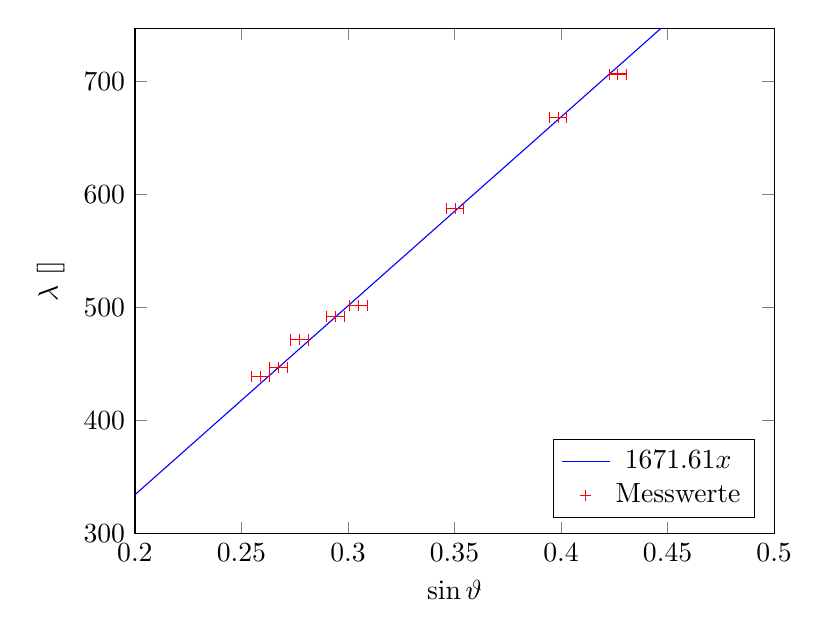
\begin{tikzpicture}
\begin{axis}[xmin = 0.2, ymin = 300, xmax = .5,
	legend pos = south east, width = .8\textwidth, height = 8cm,
	xlabel = $ \sin\vartheta $,
	ylabel = {$ \lambda $ [\si{\nano\meter}]}]
	
	\addplot+[no marks, ] {1671.61*x};
	\addplot+[mark = +,only marks, error bars/.cd, x dir = both, x explicit,] table[x=x,y=y, x error = xerr] {
y	x	xerr
438.8	0.2588190451	0.0042146465
447.1	0.2672383761	0.004204631
471.3	0.2773146533	0.0041921899
492.2	0.2940403252	0.0041704338
501.5	0.304864299	0.0041556106
587.5	0.3502073813	0.0040870034
667.8	0.3987490689	0.0040014294
706.5	0.4265687399	0.0039464301
};
\legend{{$ \num{1671.61}x $}, Messwerte}
\end{axis}
\end{tikzpicture}
	\caption{Eichkurve}
	\label{fig:kalib}
\end{figure}

\newpage
\section{Diskussion} 
